%
% $RCSfile: layer_supertype.tex,v $
%
% Copyright (C) 2002-2008. Christian Heller.
%
% Permission is granted to copy, distribute and/or modify this document
% under the terms of the GNU Free Documentation License, Version 1.1 or
% any later version published by the Free Software Foundation; with no
% Invariant Sections, with no Front-Cover Texts and with no Back-Cover
% Texts. A copy of the license is included in the section entitled
% "GNU Free Documentation License".
%
% http://www.cybop.net
% - Cybernetics Oriented Programming -
%
% http://www.resmedicinae.org
% - Information in Medicine -
%
% Version: $Revision: 1.1 $ $Date: 2008-08-19 20:41:07 $ $Author: christian $
% Authors: Christian Heller <christian.heller@tuxtax.de>
%

\subsubsection{Layer Supertype}
\label{layer_supertype_heading}
\index{Layer Supertype Pattern}

The \emph{Layer Supertype} pattern \cite{fowler2002} is a rather simple but
quite useful one. It assumes that a system is structured using the
\emph{Layers} pattern. What the pattern proposes is to add a (possibly
abstract) class that all other classes in its layer inherit from (figure
\ref{supertype_figure}). The reason is that basic functionality common to all
classes in a layer, for example persistence- or logging capabilities, can be
provided once by the supertype, such avoiding redundancies.

\begin{figure}[ht]
    \begin{center}
        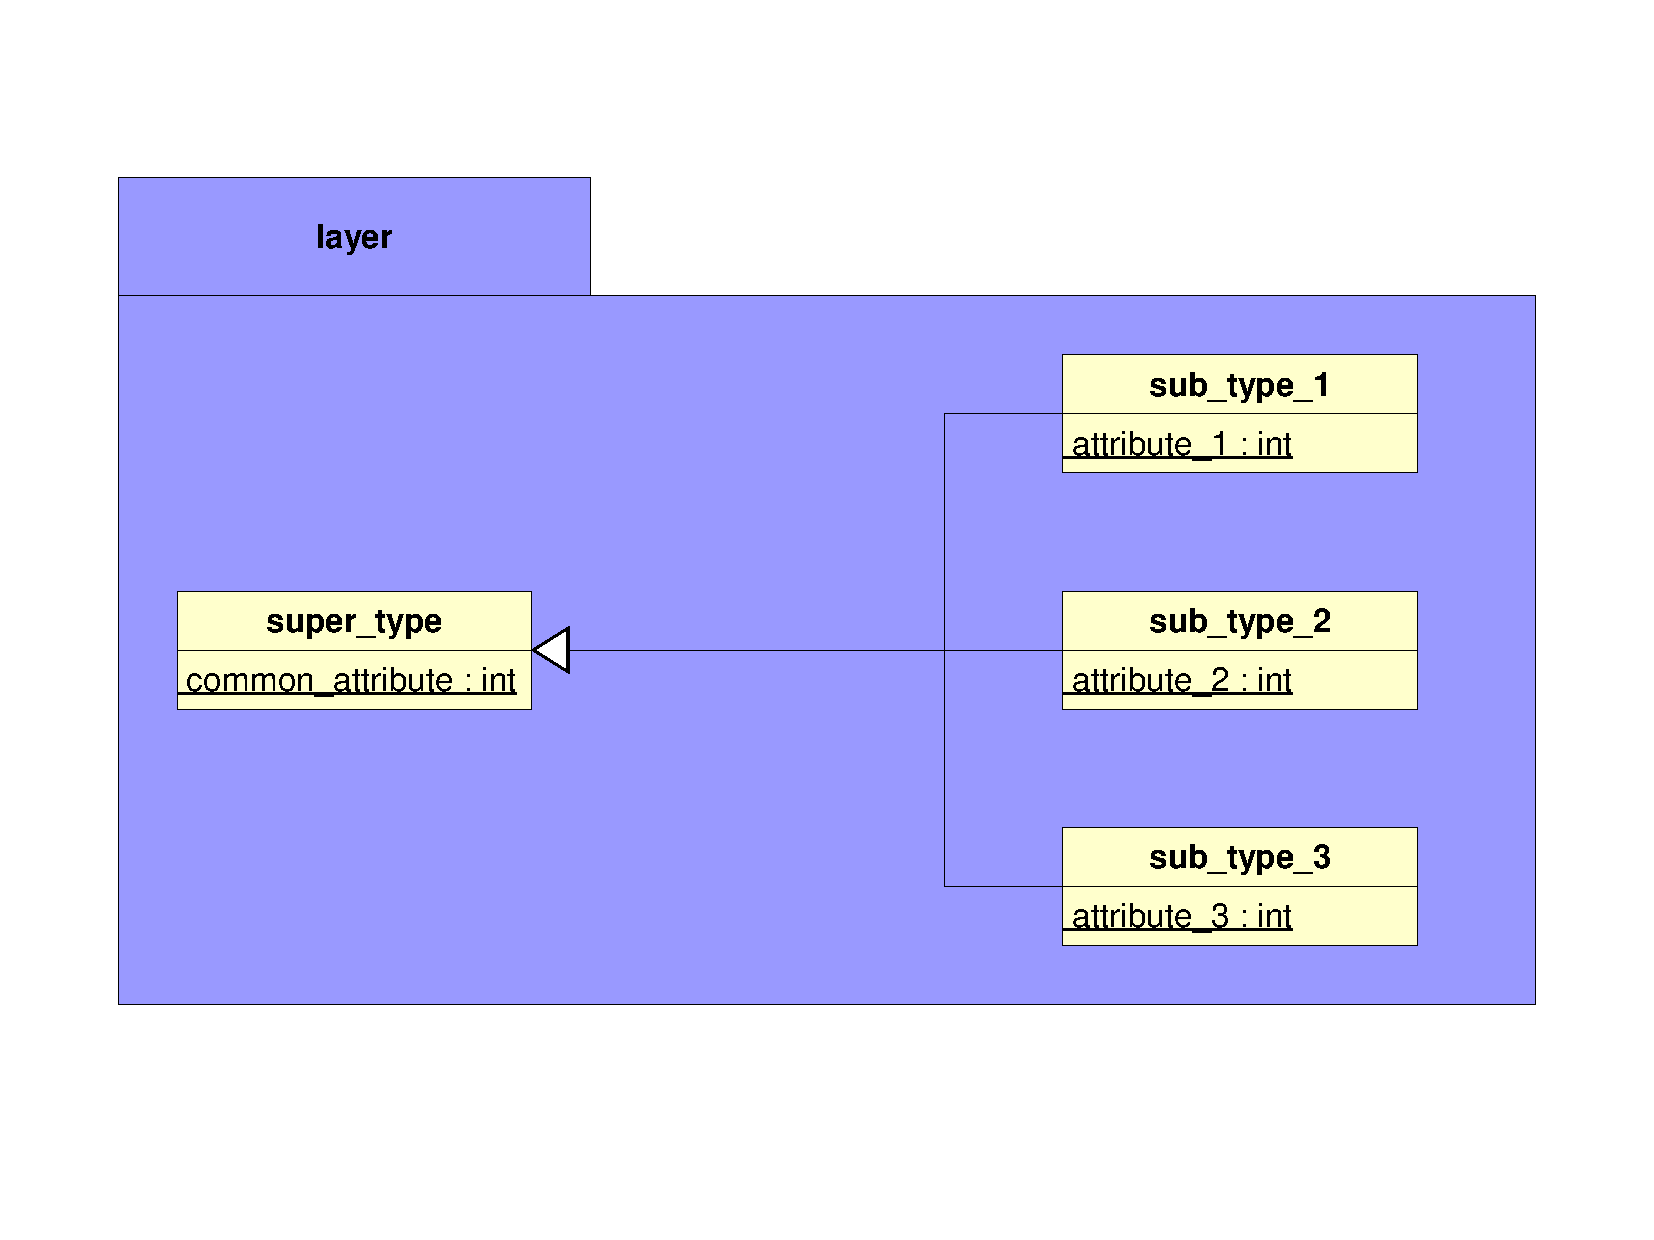
\includegraphics[scale=0.3,angle=-90]{graphic/supertype.pdf}
        \caption{Layer Supertype Pattern}
        \label{supertype_figure}
    \end{center}
\end{figure}

The language introduced in chapter \ref{cybernetics_oriented_language_heading}
does not use inheritance and thus cannot use super knowledge templates in the
meaning of the \emph{Layer Supertype} pattern. Nevertheless, the pattern is important
because of its idea to categorise similar knowledge, such as all templates of:
a \emph{Textual User Interface} (TUI), a \emph{Graphical User Interface} (GUI),
a \emph{Domain Model} etc.
